%%Berichtvorlage für EDBV WS 2015/2016

\documentclass[deutsch]{scrartcl}
\usepackage[top=1cm,left=1cm,right=1cm,bottom=1cm]{geometry}
\usepackage[ngerman]{babel}
\usepackage[utf8]{inputenc}
\usepackage{algorithmic}
\usepackage{algorithm}
\usepackage{graphicx}
\usepackage{amsmath,amssymb}
\usepackage{subcaption}
\captionsetup{compatibility=false}
\usepackage{multirow}
\usepackage{color}

\begin{document}

\title{Schnaps\"onig} %%Projekttitel hier eintragen

%%Namen und Matrikelnummern der Gruppenmitglieder hier eintragen
\author{Jan Michael Lajarno (01425799)\\
Andreas Brunner (01429369)\\
Miran Jank (01526438)\\
Thorsten Korpitsch (01529243)\\
Aleksandar Marinkovic (01634028)}
\date{\vspace{-5ex}}



%%------------------------------------------------------

\maketitle

\begin{figure}[h!]
	\centering
	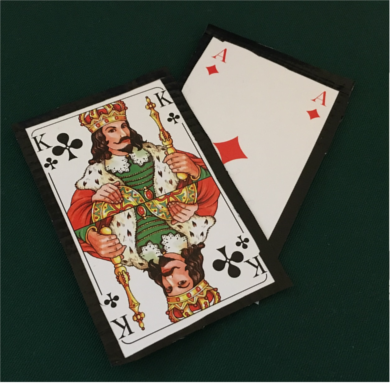
\includegraphics[width=0.3\textwidth]{titelbild.png}
	\caption{Spielzug beim Schnappsen als Eingabe}
	\label{fig:erg}
\end{figure}

%%------------------------------------------------------

\section*{Projekt}
Nach jedem Spielzug beim Schnappsen wird ein Bild (siehe Abbildung 1) als Eingabe verwedet. 
Wir analysieren dieses Bild, berechnen den Gewinner des Spielzugs und die Punkte die er gewonnen hat.

\section*{Vorgangsweise}

Beschreibung der Pipeline

\begin{enumerate}
	\item In einer Schleife werden die Bilder aus einem Ordner gelesen
	\item Die Bilder werden in ein Graustufenbild umgewandelt und dann mit Otsus Methode in ein Bin\"arbild umgewandelt
	\item Die 2 Karten werden mittels Zusammenhangskomponenten getrennt
	\item Die Fl\"ache der erhaltenen Karten gibt an welche die Obere und welche die Untere ist
	\item Die Karten werden mittels Geometrischer Transformation hochkannt gestellt und von perspektivischer Ansicht in die Orthogonale Ansicht gebracht
	\item Die Karten werden mit Hilfe des Template-Matchings (Korrelation) identifiziert
	\item Der Gewinner des Spielzugs wird ermittelt und die Punkte gutgeschrieben und auf die Konsole ausgegeben
	\item Der Gesamtgewinner wird in der Konsole ausgegeben

\end{enumerate}

\section*{Ergebnisse}

Das Ergebnis erfolg in textueller Form und kann so aussehen:\\
Spielzug 1: Ass(Karo) gegen K\"onig(Karo). Spieler 1 gewinnt 15 Punkte.\\




\end{document}
